\documentclass[titlepage]{scrartcl}
\usepackage{enumitem}
\usepackage[british]{babel}
\usepackage[style=apa, backend=biber]{biblatex}
\DeclareLanguageMapping{british}{british-apa}
\usepackage{url}
\usepackage{float}
\restylefloat{table}
\usepackage{perpage}
\MakePerPage{footnote}
\usepackage{abstract}
\usepackage{graphicx}
% Create hyperlinks in bibliography
\usepackage{hyperref}
\usepackage{amsmath}

\usepackage[T1]{fontenc}
\usepackage[utf8]{inputenc}
\usepackage{blindtext}
\setkomafont{disposition}{\normalfont\bfseries}

\graphicspath{
    {./resources/},
}
\addbibresource{~/PerryPerrySource/LaTeX/ExperimentalMusic_Bibliography.bib}

\newsavebox{\abstractbox}
\renewenvironment{abstract}
  {\begin{lrbox}{0}\begin{minipage}{\textwidth}
   \begin{center}\normalfont\sectfont\abstractname\end{center}\quotation}
  {\endquotation\end{minipage}\end{lrbox}%
   \global\setbox\abstractbox=\box0 }

\usepackage{etoolbox}
\makeatletter
\expandafter\patchcmd\csname\string\maketitle\endcsname
  {\vskip\z@\@plus3fill}
  {\vskip\z@\@plus2fill\box\abstractbox\vskip\z@\@plus1fill}
  {}{}
\makeatother

\DeclareCiteCommand{\citeyearpar}
    {}
    {\mkbibparens{\bibhyperref{\printdate}}}
    {\multicitedelim}
    {}

\begin{document}
    \title{Experimental Music\\Summative Assignment 2\\Essay}
    \subtitle{\LARGE{The role of electronic feedback and amplification in
    experimental music composition.}}
    \author{Sam Perry\\U1265119}
    \date{}

    \begin{abstract} 
        The use of electronic feedback as a tool for musical composition has
        featured in many compositions, popular for it's complex, volatile and
        indeterminate nature.  Intrinsic to the use of feedback is the use of
        amplification, capable of artificially altering an input's energy, as a
        method for feedback control. This essay aims to provide a definition of
        these tools in their different forms, and to analyse their use in a
        range of prominent compositions. Forms of feedback will be defined,
        followed by a discussion of the musical implications of their use,
        including the consideration of aspects such as process, indeterminacy,
        spectral implications and rhythmic implications. This will be related
        to a number of compositions in order to provide an overall
        understanding of their role in experimental music composition.
    \end{abstract}

    \maketitle

    \section{Defining feedback and amplification}
    A simple definition of feedback is the process of routing the output of a
    system back to the input of that system.~\parencite[p.1]{weisert2010ioi}
    This can take many forms in the context of music. Whether it is the acoustic
    feedback created by aiming a microphone to it's amplifier, or the digital
    feedback present in an IIR filter, in all cases a loop is created from an
    output point of a system, back to it's input.\\
    The two types of feedback to be discussed are:
    \begin{itemize}
        \item{Acoustic Feedback}
        \item{Electronic Feedback}
    \end{itemize}
    In order to fully understand feedback, electronic amplification will also
    be explored due to it's integral part in feedback system control.
        
    \subsection{Acoustic Feedback}
    Acoustic feedback occurs when a closed loop is created between an audio
    transducer (such as a microphone or guitar pick-up) and amplifier,
    causing previously amplified audio to be re-amplified continuously at an
    exponential rate, as illustrated in Figure~\ref{acoustic_feedback}.
    \begin{figure}[H]
        \makebox[\textwidth]{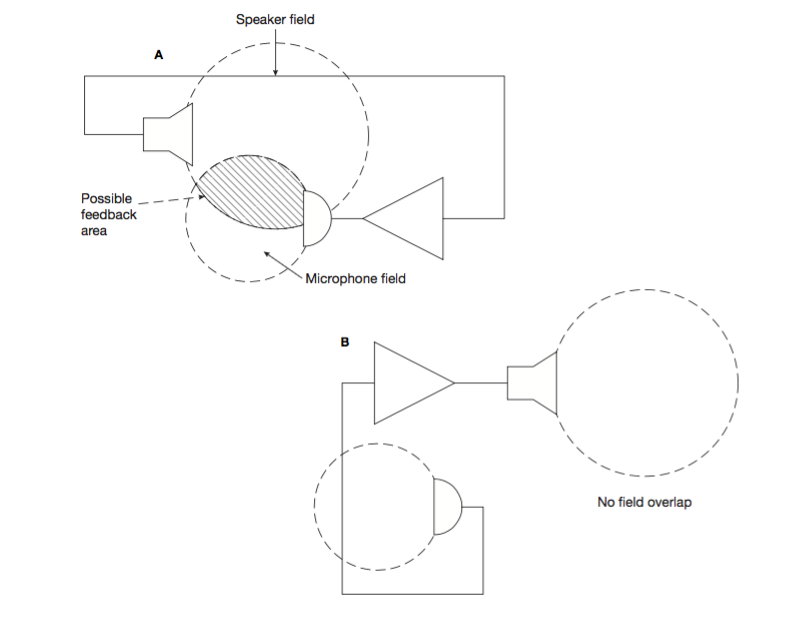
\includegraphics[width=0.75\textwidth]{acoustic_feedback_diagram}}
        \caption[Caption for LOF]{Acoustic Feedback Diagram\protect\footnotemark}
        \label{acoustic_feedback}
    \end{figure}

    \footnotetext{Diagram taken from:~\parencite[p.185]{holmes2012eaem}}

    The volatile and unpredictable nature of acoustic feedback has been used to
    great effect in both popular and avant-garde
    music.~\parencite[p.186]{holmes2012eaem} Pioneering guitarists such as Jimi
    Hendrix have used the loop created through placing an electric guitar
    pickup close to it's amplifier to compliment virtuosic guitar solos in
    pieces such as Foxey Lady~\citeyearpar{hendrix1967fl}. This is taken one
    step further in avant-garde works such as Steve Reich's Pendulum Music,
    where feedback becomes the focus of the piece entirely. This is discussed
    further in section~\ref{pendulum}
    
    \subsection{Electronic Feedback}
    Electronic feedback takes the principal of recursively feeding an output
    back into an input into the analog electronics domain. In this situation,
    the recursive processing is performed purely on electrical signals,
    replacing the initial acoustic input from the microphone found in acoustic
    feedback, with a purely electronic input as part of an electronic circuit.
    The result of this process is then produced in the listening space via
    amplification~\parencite[p.187]{holmes2012eaem}. Composers such as David
    Tudor and Gordon Mumma explore these techniques through their creation and
    use of custom electronics designed to exploit the characteristics
    of this effect.~\parencite[p.186, 390]{holmes2012eaem} A detailed analysis
    of these techniques are presented in section~\ref{ElecFeed}

    \subsection{Amplification}
    Amplification is the process of scaling a signal by a chosen factor.~\parencite[p.3-4]{kadis2012sosr}. 
    This artificial modification of amplitude has a number of interesting sonic
    effects in itself, as it allows for the magnification of sounds that may not
    naturally be perceivable and conversely, the reduction of extremely loud
    sounds to a comfortable range for hearing. This is explored through
    works such as John Cage's Cartridge Music as discussed in
    section~\ref{amp}\\

    It has been stated that feedback is difficult to control. This is due to
    it's recursive nature and the tendency for output that exceeds unity gain
    (a state, whereby the output amplitude of a feedback system is equal to
    that of it's input) to be fed back into the system.  Amplification is
    therefore a crucial element for controlling the results of a feedback
    system. By attenuating an output before feeding it back to a system, it is
    possible to ensure that outputs do not grow at an exponential
    rate.~\parencite[p.71-72]{zolzer2011dafx}
    \begin{figure}[H]
        \makebox[\textwidth]{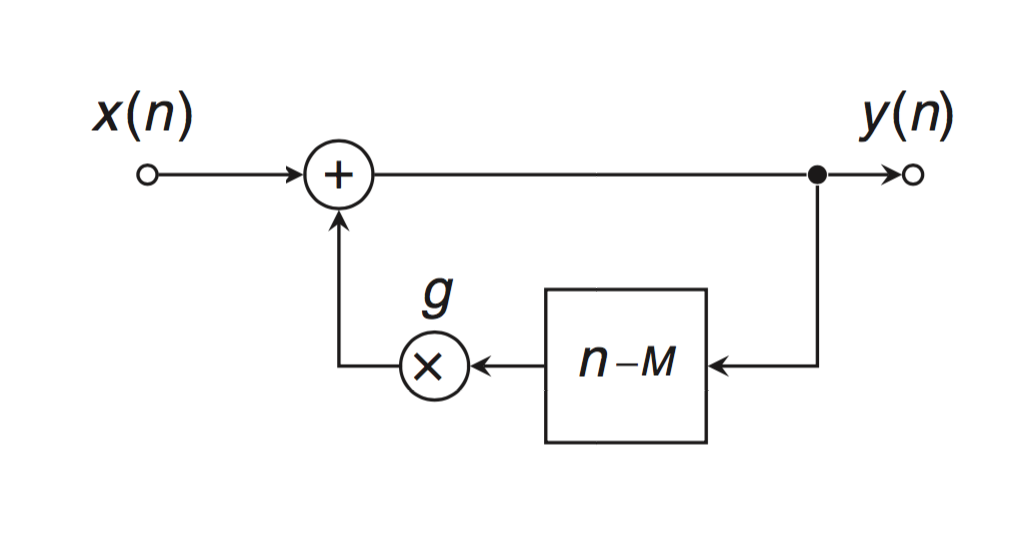
\includegraphics[width=0.75\textwidth]{IIR_flow_diagram}}
        \caption[Caption for LOF]{Basic Feedback Signal Flowchart\protect\footnotemark}
        \label{feed_flowchart}
    \end{figure}

    \footnotetext{Diagram adapted from:~\parencite[p.72]{zolzer2011dafx}}

    \begin{figure}[H]
    This can be demonstrated mathematically using the following example equation
    for a feedback system as illustrated in figure~\ref{feed_flowchart}~\parencite[p.70-72]{zolzer2011dafx}:
        \begin{align*}
            & y(n) = x(n) + gy(n-M)\\
            & \text{where:}\\
            & x\text{ is the input signal}\\
            & y\text{ is the output signal}\\
            & n\text{ is the current point in time}\\
            & M\text{ is the signal delay in time}\\
            & g\text{ is the feedback coefficient}\\
        \end{align*}
    \end{figure}

    \section{Musical Aspects and Implications of Feedback Systems}
    There are a number of interesting musical implications when using feedback
    and amplitude adjustment as a compositional tools. Features such as
    indeterministic and rhythmic characteristics, inherent to the nature
    of feedback, make it an interesting technique for musical exploration and
    there are many examples of artists exploiting these qualities in
    experimental compositions. Likewise, amplitude modification offers a number
    of compositional possibilities for both the control of feedback and for
    creative effect in of itself. This section outlines some of the key musical
    aspects of feedback and artificial amplification and provides examples of
    notable compositions that demonstrate these principals.

    \subsection{Indeterminacy}\label{indeterminate}
    Indeterminacy is related to the use of chance operations in music
    composition and performance. Techniques that involve a degree of
    uncertainty, where external variables or unpredictable factors affect the
    outcome, are defined as indeterminate. Simms uses the following definition
    for indeterminacy:
    ``Any part of a musical work is indeterminate if it is chosen by chance, or
    if its performance is not precisely
    specified.''~\parencite[p.357]{simms1986mtc} It is a topic of interest for
    experimental composers for a number of reasons.

    \subsubsection{Variation in Performance}\label{variance}
    Using indeterministic processes as part of a composition allows for
    variation in the performance of said composition on a case by case basis.
    Through the addition of random factors to a composition, far greater
    degrees of variance are created in the performance of a piece, allowing for
    an infinite number of possible versions as opposed to the comparatively
    limited interpretation of static compositions where all elements are
    controlled directly by the composer.~\parencite[p.97-98, 381]{jc2009co,
    holmes2012eaem}
    This variance can take many forms dependant on the indeterministic factor.
    An example might be the performer, which is demonstrated well through
    Cornelius Cardew and Christian Wolff's compositions for the Fluxorchestra.
    By composing ``unambiguous, concrete proposals (which still left room for
    personal idiosyncrasies in realization)'', indeterminicity was created
    through the skill and interpretation of the performers in pieces such as
    ``Stones'' by Wolff or ``The Great Learning'' by
    Cardew~\parencite[110]{nyman1999em}\\
    In terms of feedback, variance in feedback will depend primarily on the
    variance of the input to the system and the variance of control. Due to the
    non-linear fashion in which feedback effects input to produce an output,
    subtle changes in these may result in significant changes to the output. An
    example of this is a guitarist using an amplifier to produce feedback from
    his guitar. In each performance, the subtle changes in distance between the
    guitar and amplifier may result in significant differences to feedback
    tone. This property of feedback applies to compositions such as Steve
    Reich's Pendulum Music and Gordon Mumma's Hornpipe, discussed in
    section~\ref{pendulum} and section~\ref{hornpipe}.

    \subsubsection{Bias Removal}
    Indeterminacy is able to remove personal bias and ego involved in decision
    making from a composition or performance. By leaving compositional
    decisions to chance, it is ensured that the music produced is not created
    with intent and is separated from the composer's personal taste, as stated
    by John Cage~\parencite[p.381]{holmes2012eaem}. This technique is used in
    his composition ``Music of Changes'', where chance operations are used for
    the organisation of material in such a way that ``bypassed a reliance on his
    aesthetic judgement''. By combining this relinquished control with the
    precise control of other aspects of the piece, Cage was able to create a
    ``balance between rational and irrational'' through the combination of
    control and total removal of control over compositional
    elements~\parencite[p.97-98]{jc2009co}.\\
    In relation to feedback directly, the ability for feedback to create
    exponentially complex output from relatively simple feedback systems
    create clear elements of indeterminacy through the unpredictability of
    their output. This is demonstrated in Steve Reich's ``Pendulum Music'' as
    discussed in section~\ref{pendulum}. Parallels can be drawn between John
    Cage's use of indeterminacy to dictate organizational aspects of ``Music of
    Changes''~\citeyearpar{cage1951mfc} with Steve Reich's use of feedback to dictate sonic events in
    ``Pendulum Music''.\\
    Feedback builds on methods such as Cage's use of the I Ching as far greater
    quantity of unpredictable events can be generated quickly, compared to the
    manual ``brute-force'' approach of generating each event as is the case
    with the I Ching. 
    \subsection{Process and Control}
    The term ``process'' refers to the situation outlined by a composer,
    designed for the creation of sound. Where popular music focuses on creating
    pre-defined musical content and structure, experimental musicians typically focus on
    the creation of a process through which sound may be generated. This may
    involve the creation of rules or instructions that outline the conditions
    that are needed in order to create an outcome, the content of which may
    differ on each performance based on any indeterministic factors (see
    section~\ref{indeterminate}) There are many forms of process used for the
    composition of experimental music. These are observed in detail in
    \textit{Experimental Music - Cage and
    Beyond}~\parencite[p.4-14]{nyman1999em}

    \subsubsection{Feedback Process}
    Feedback is concerned mainly with electronic process, where an electronic
    system is defined/set up in order to facilitate the creation of sound. The
    specified setup will therefore have a direct impact on the outcome of the
    piece, combined with other factors such as the methods used for control of other
    processes involved in the piece's realisation. This is true of Gordon
    Mumma's Hornpipe~\citeyearpar{mumma2002lem} (as detailed in
    section~\ref{hornpipe}) where electronic circuitry is designed specifically
    to explore the effects of using custom electronic circuitry to produce
    controlled feedback~\parencite[p.8, 390]{nyman1999em}

    \subsubsection{Feedback Control}
    As stated previously, feedback can be difficult to control due to it's
    indeterministic properties. The complex and intricate outputs possible with
    even the simplest of feedback systems causes results to differ
    significantly based on the exact conditions of the system. The two most
    significant factors that affect a basic feedback system are:
    \begin{itemize}
        \item System input
        \item System parameters
    \end{itemize}

    \paragraph{System Input}\mbox{}\\ 
    As with most systems, an alteration to the input of the system will result
    in the alteration of the output. This is generally true of feedback systems
    as, for example, providing an electronic feedback circuit with a louder
    input will most likely result in a louder output. This relationship may not
    be linear and depends on the design of the feedback system, which in turn
    dictates the indeterministic nature of these
    systems~\parencite[p.19-27]{weisert2010ioi}. However, it still provides a
    method for control over the output of the system. This is apparent in
    Mumma's Hornpipe~\citeyearpar{mumma2002lem} where the performer must adapt
    the input to the system (in this case the sound produced by the French
    horn) in reaction to the electronic sound produced by the ``cybersonic
    console''.
    
    \paragraph{System Parameters}\mbox{}\\
    As stated above, the design of the feedback system will determine it's
    response to a given input. A common method for controlling the design of a
    feedback system is through the implementation of variable nodes for the
    dynamic adjustment of parameters.~\parencite[p.19-27]{weisert2010ioi}
    A clear example of this is the use of a scaling factor in the feedback loop
    to parametrize the regenerative/degenerative nature of the system. By
    altering this parameter, the degree to which a signal is
    amplified/attenuated on each recursion can be modified dynamically during
    performance. This would be attributed to the guitar-amplifier distance in
    the typical guitar feedback example mentioned in section~\ref{variance}

    \subsection{Rhythmic/Temporal Implications of Feedback}
    The process of feeding a signal back through a system has consequences in
    terms of a subsequent iteration's rhythms. The superposition of signals
    causes alterations in the temporal content of the subsequent signals,
    resulting in the removal and addition of temporal peaks to the signal (a
    signal's peaks are linked to the perceived characteristic of the signal's
    rhythm).  The effects of feedback are discussed at length with regards to
    Alvin Lucier's ``I am sitting in a room'' by 
    Weisert~\parencite[p.64-68]{weisert2010ioi}. The rhythmic impact of a
    feedback system is complex. However, at a basic level, it should be
    understood that feedback causes a shift in rhythmic content over time.  The
    exact rhythmic alteration is dependant on factors such as the feedback
    system, input signal and it's relationship with the subsequent iterations
    of itself. This is explored extensively in David Tudor's Pulsers (see
    section~\ref{tudor})

    \subsection{Spectral Implications of Feedback}
    As with rhythmic content, feedback has a complex effect on the spectral
    content of a signal. As with the rhythmic content, the effect of
    superposition on the original signal emphasizes and reduces spectral
    content. This is again, examined at length in Weisert's analysis of ``I am
    sitting in a room'' and a similar shift in spectral content can be observed
    to that of the rhythmic content over
    time.~\parencite[p.60-64]{weisert2010ioi}
    
    \subsection{Dynamic Implications of Artificial Amplitude Adjustment}
    The artificial adjustment of audio amplitude is an important technique as it
    allows for the alteration of a signal's energy. This acts as a form of
    sonic magnifier, able to make inaudibly small sounds audible, as
    demonstrated in pieces such as John Cage's ``Cartridge
    Music''~\citeyearpar{cage2013cm} and Stockhausen's ``Mikrophonie''
    collection~\citeyearpar{stockhausen1995mmt}. This technique was instrumental in the
    development of electroacoustic music by artists such as Cage and
    Stockhausen as it allowed the details of quiet sounds to be amplified
    artificially in a live environment.~\parencite[p.351-352]{holmes2012eaem}

    This process is combined with the principals of a feedback system in order
    to provide control to a feedback system. By altering the amplification of
    signals in a feedback system, dynamic control of feedback properties is
    possible. This is clearly used in works such as Robert Ashley's ``The
    Wolfman'' in order to tune the feedback in an appropriate
    fashion.~\parencite[p.186]{holmes2012eaem}

    \section{Composition Analysis}
    There are a large number of pieces that utilise electronic feedback and
    amplification creatively. This section analyses some of the most prominent
    pieces in order to present some explorations and usages of feedback in
    experimental music.

    \subsection{Amplification}\label{amp}
    \subsubsection{John Cage's Cartridge Music~\citeyearpar{cage2013cm}} 
    Cartridge music explores the amplification of small sounds through the use
    of phonograph cartridges and a range of object in order to create amplified
    audio based on the performer's interactions with these objects. By
    inserting the object in place of the phonograph's needle, a performer is
    able to create amplified sounds that vary based on the type of object used.
    This piece was created to explore the possibilities of amplifying small
    sounds to within an audible range and the chance sounds that are created as
    a result.  The piece focuses on the aesthetics of different mediums of
    object, and does not concern itself with player improvisation as do other
    examples. This reflects Cage's attitude towards the process and openness to
    chance events by allowing the unexpected to form part of the piece, without
    intervention of the performer.~\parencite[p.56-61]{lucier2012m109}

    \subsection{Acoustic Feedback}
    \subsubsection{Steve Reich's Pendulum Music~\parencite[p.31]{reich2002wom}}\label{pendulum} 
    This piece is possibly one of the most direct explorations of acoustic
    feedback. Where other pieces explore the effects of feedback on/with an external source,
    Pendulum Music focuses directly on the sonic phenomena generated purely by
    the feedback system and the acoustics of the space~\parencite[p.50-51]{weisert2010ioi}.

    Aesthetically, the piece begins with clear rhythms created by the distinct
    motion of the microphones as they pass over the speakers. This slowly
    degrades as the microphones lose momentum, resulting in the pure feedback
    tones created as the microphones hang motionless over the speaker at the
    end. Interesting phase relationships can be observed between the
    microphones as the piece progresses, which is in keeping with Reich's works
    such as Come Out~\citeyearpar{reich1966comeout}

    This piece has a clear focus on process and was described as ``the ultimate
    process piece'' by Reich. Realised as an ``audible sculpture'', the piece is
    designed to limit human interaction in order to focus on the natural
    interaction of acoustic feedback. Control of aesthetics is determined by
    the semi-indeterministic method of releasing the suspended microphones,
    then allowing natural swinging motions to dictate sonic events and rhythms.
    This process is described as semi indeterministic, as it is clear that the
    microphones will swing back and fourth at diminishing amounts over time,
    however the audible feedback, interplay between audible events, feedback
    tone etc\ldots are largely left to chance. This created a stark contrast
    between the compositional process and chaos process presented through the
    uncontrolled feedback~\parencite[p.186]{holmes2012eaem}.

    This piece fits in with reich's other work through it's exploration of theme
    such as audio phaseing and rhythm, similar to that of his works such as Come
    Out~\citeyearpar{reich1966comeout} and Clapping Music~\citeyearpar{reich1966clap}
    
    \subsubsection{Robert Ashley's The Wolfman~\citeyearpar{ashley2003w}}\label{wolfman} 
    
    The Wolfman explores a number of aspects of acoustic feedback through the
    use of vocalisms for the control of tape sample modulated feedback. By
    creating even small vocal sounds, the performer is able to control the
    aesthetics of the feedback loop demonstrating the exponentially complex
    impact of even the simplest inputs to a feedback system, as described
    previously. Ashley commented that ``the vocal sounds used to induce the
    feedback have to be extremely soft so as not to block it'' and he regretted
    that the piece was believed to be generated by screams, which was far from
    true~\parencite[p.37]{gann2012ra}. The result is a massive build up of
    distortion and noise that develops as more vocalisms are supplied to the
    feedback loop. It has also been observed that the piece's spectral content
    is largely dictated by the room acoustics, tending towards a build up of
    high pitched, shrill tones in smaller rooms. This shows the general focus
    on the concept of process in experimental
    compositions~\parencite[p.18]{cage2011silence} as the piece may differ
    dramatically based on the conditions of the performance.

    \subsection{Electronic Feedback}\label{ElecFeed}
    \subsubsection{David Tutor's Untitled~\citeyearpar{tudor1996twfle} and Pulsers~\citeyearpar{tudor1996twfle}}\label{tudor}
    Tudor's Three Works for Live Electronics aimed to explore the creative
    possibilities of using live electronics for composition. This was achieved
    by creating custom electronic circuitry for the generation, manipulation
    and feedback of audio. This was then controlled through the live filtering
    and amplification of the feedback circuits to alter the output over
    time~\parencite[p.187]{holmes2012eaem}.
    
    \paragraph{Pulsers}\mbox{}\\
    Pulsers aimed to explore the temporal and rhythmic effect of feedback and
    live electronics by using extensive electronic feedback/amplification
    networks to modify the sound of various materials such as a tape recording
    of an electronic violin~\parencite{tudor1984twle}. By altering the amplification and filtering of the
    circuit live, the performer is given control over the rhythmic aspects of
    the output. This results in the controlled use of the complex rhythms
    possible with feedback.
    Pulsers focused primarily on the aesthetic potential of manipulating analog
    circuitry, particularly on the rhythmic impact of altering analog
    components.
    
    \paragraph{Untitled}\mbox{}\\
    Untitled was created as an exploration of the use of ``no-input'' live
    electronics. The electronic setup consisted of a complicated feedback setup
    designed to manipulate the characteristics of sounds created purely through
    the electronics (without any external input from microphones or
    recordings).
    The live adjustment of electronic parameters created an interesting
    improvisational element in Untitled, as the complex nature of the
    circuitry created an interplay between performer and the system. The
    performer would adjust parameters, the system would respond, and subsequent
    alterations would be made as a result~\parencite{tudor1984twle}.
    However, the tendency for feedback to become uncontrollable and the
    extremely complex signal path resulted in a piece too complex to be
    manageable in terms of live performance. This is a good example of the
    indeterminate, complex nature of
    feedback.~\parencite[p.83-85]{weisert2010ioi}
    This piece served as an attempt to explore the musical possibilities
    created purely from the sound of the electronics themselves. This differed
    from the conventional use of electronics to alter an external sound created
    by an oscillator or external audio source.~\parencite{tudor1984twle}

    \subsubsection{Gordon Mumma's Hornpipe~\citeyearpar{mumma2002lem}}\label{hornpipe}
    Hornpipe is a composition that combines the input from a French horn with
    custom electronic circuitry created by Mumma, in order to transform the input by
    monitoring and altering output based on input resonance. 
    The piece aims to explore electronic circuitry as a form of extension to
    the horn, as electronic characteristics are dependant on the input from the
    horn and the acoustic space in which the piece is
    performed.~\parencite[p.101-103]{nyman1999em}
    This piece demonstrates a combination of electronic and human process as
    the sound produced by the electronic circuitry's interplay with the human
    improvisation in reaction creates the final result.
    The piece also explored the indeterministic aspects of feedback due to the
    unpredictability of the electronic circuitry based on the number of factors
    that determine it's output.

    \section{Conclusion}
    It is clear that feedback provides enormous potential for creative
    possibilities in music, as demonstrated by the wide variety of
    experimental compositions detailed. This is far from an exhaustive set of
    examples and many more examples explore the unique properties of feedback.
    Overall, feedback's indeterministic nature, spectral/temporal impact, and
    range of possibilities for control make it a unique and interesting area
    for musical experimentation.

    \printbibliography

\end{document}
